\chapter{Time Delay Compensation and Predictive Display}
\label{ch_7:PDsply}
In the last chapter it was shown using simulation results that time delay between the remote and local station leads the system towards instability. In this chapter we first present predictive model controller for time delayed teleoperation. WE then highlight the issues of time delay on human performance. We then present our  RGB-Depth sensor based  predictive display implemented in our system  to alleviate the problem of time delay in visual feedback.

\section {Model Based Time Delay Compensation}
As shown in the last chapter, simulation of time delays system with pure pursuit model for human controller in stability starts with as the delay in feedback i.e input delay to the human model increase. In paper by Ollero \cite{ollero1995stability} stability of pure pursuit with input delay was presented. The kinematic model shown in Equation \ref{eqn:ppRobotModel}  and first order model for steering dynamics for the vehicle was assumed. 
\begin{equation}
\label{eqn:ppRobotModel}
\begin{pmatrix}
\dot{x'}_w\\ \dot{y'}_w\\ \dot{\theta}
\end{pmatrix}
=
\begin{pmatrix}
-V \sin\theta\\ V\cos\theta\\V\gamma
\end{pmatrix}
\end{equation}
\begin{equation}
\label{eqn:ppSteering}
\frac{d\gamma'}{dt}=-\frac{1}{T}(\gamma'-\gamma_R)
\end{equation}
where, $(x',y',\theta)$ is the posture of robot in coordinate system attached to the robot,  $V$  is the longitudinal velocity,  $\gamma$ is the angular velocity, $T$ time constant of steering dynamics and $\gamma_r$ the control input.  Since the control input is generated by Pure Pursuit it is given by
\begin{eqnarray}
\gamma_r=\frac{1}{r}=\frac{2x}{L^2}
\end{eqnarray} 
 where $r$ is defined in Equation \ref{ppControl} and $L$ is the \textit{look ahead distance}. The above Equations \ref{eqn:ppRobotModel} and \ref{eqn:ppSteering}  using the fact that $\dot{y'}_w=0$, because of the non-holonomic constrain of the robot, can be written  in the form of state space  form  as 
\begin{equation}
	\begin{pmatrix}
	\dot{x}\\\dot{\theta}\\\dot{\gamma}
	\end{pmatrix}
	=
	\begin{pmatrix}
	-\sin\theta\\ \gamma \\ -\gamma -\frac{2x}{l^2}
	\end{pmatrix}
\end{equation}
where the following scaling of variables were used to render it non-dimensional. 
\begin{equation*}
	t=\frac{t'}{T}, \quad x=\frac{x'_w}{VT}, \quad \gamma=VT\gamma',\quad l=\frac{L}{VT}
\end{equation*}
The above system was linearised about the origin and  delay $\tau$ in  input was introduced  to get Equation \ref{equ:delayPP}
 \begin{equation}
 \label{eqn:delayPP}
 \begin{pmatrix}
 \dot{x}\\\dot{\theta}\\\dot{\gamma}
 \end{pmatrix}
 =J
 \begin{pmatrix}
 x(t)\\\theta(t)\\\gamma(t)
 \end{pmatrix}+
 J_\tau 
  \begin{pmatrix}
 x(t-\tau)\\\theta(t-\tau)\\\gamma(t-\tau)
 \end{pmatrix}
 \end{equation}
 where $J$ is the Jacobian with respect to state and $J_\tau$ is Jacobian with respect to $\tau$. 
 Based on location of roots of the Characteristic Quasi-Polynomial $q(s)=det[sI-J-J_\tau~ e^{s\tau} ] $, a graphical result for different input delay a limiting  look ahead distance for stable path tracking was presented for a  circular path. In view of the above a stabilizing controller design is needed, which is presented next.
 \begin{figure}
 	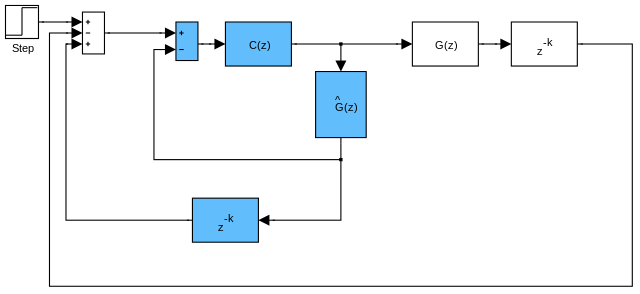
\includegraphics[width=\linewidth]{Chapter7/fig/Smith_predictor}
 	\caption{Smith Predictor}
 	\label{fig:Smith}
 \end{figure}
 
 One of the earliest controller for Linear system with time delay is the Smith Controller \cite{smith1959controller}. The schematic of the smith controller is shown in figure \ref{fig:Smith}. As can be seen there are two loops the inner and the outer loop. Where $G(z)$ is the plant, $C(z)$ is the stabilizing controller  for plant with out delay, $\hat{G}(z)$ is the model of the plant. 
 As can be seen from the figure \ref{fig:Smith} thet during the period (k unit of time) when the feedback (output) is not available the model of the plant is used to predict the actual plant behaviour and generate the control signal accordingly. 
 
 In our case the plant is the mobile robot. As shown in Figure \ref{fig:SmithRobot} the 

  
 \begin{figure}
 	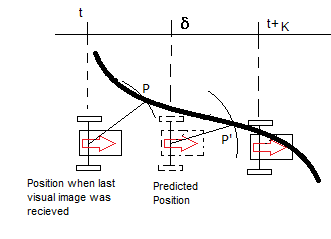
\includegraphics{Chapter7/fig/robotPredictPos}
 	\caption{Smith predictor applied to mobile robot}
 	\label{fig:SmithRobot}
 \end{figure}
  
\section{Predictive Display}
Predictive display has been defined as using the computer for extrapolating the display forward in time \cite{sheridan}. In this a local model of the remote scene is used to predict and render the remote scene in response to operator command. It replaces the delayed video feedback with extrapolated synthesised  image of the remote environment and local enables the operator to perform the task normally. 

\section{Remote Scene Extrapolation} 
The visual data present in the current frame is the view that the robot has seen $h_1$ second earlier. In order to predict the current scene that the robot might be seeing we need to estimate the current position of the robot. Once the current position of the robot is known we re-construct a view form the old scene by moving the view point to the current position of the robot. To explain this further and to use it in the teleoperation simulation model discussed in chapter 6
\subsection{here}

